% Chapter Template

\chapter{Literature Review} % Main chapter title

\label{Chapter3} % Change X to a consecutive number; for referencing this chapter elsewhere, use \ref{ChapterX}

%Typical examples of action recognition \cite{i3d} have used complex convolutional neural networks (CNNs) on the RGB frames, pulling features such as rgb flow \cite{rgbflow} in order to enhance results. This method has proved to work well, however these models often require large amounts of GPU memory and are required to be run on high end hardware, which is a potential issue when applied to real-world scenarios where the necessary hardware may not be available. In addition, background noise is much more difficult to filter out and generalizing to different environments is difficult.

%A subset of action recognition models utilize skeleton-based action recognition. These models aim to utilize the positions of joints/bones in the model in order to filter out background data, and allow the model to focus on the actual person rather than background data. Typically these involve simpler CNNs that allow for faster computation on lower quality hardware. Many different approaches are used to achieve this action recognition. \cite{potion}, \cite{PA3D} utilize processed joint heatmap images and simple 2D-CNNs. \cite{simple_yet_efficient} \cite{smaller_faster_better} use intermediate representations to construct custom image representations that can be easily processed by simple CNNs. RNNs and LSTMs \cite{two_branch_stacked_lstm} \cite{RNN_joint_relative_motion} \cite{RNN_occlusion} \cite{DS_lstm} and Transformers \cite{transformersnippets} \cite{transformertwobranch} have been used as well to obtain good results with skeleton data.

%Almost always, these skeleton based models utilize 2D pose data. There have been some examples of extracting 3D pose from depth cameras \cite{depthcamera3dpose} as well as estimating 3D pose from 2D pose \cite{3dposefrom2d} and only the RGB frames \cite{2dposefromrgb}. These techniques have been used in the past for human action recognition \cite{3dposeactionrecognition}, however 2D pose estimation is a much easier task and the models that have been used are generally much higher quality, and therefore is more reliable for the task of human action recognition.

%----------------------------------------------------------------------------------------
%	Image Classification
%----------------------------------------------------------------------------------------
\section{Image Classification}

%----------------------------------------------------------------------------------------
%	Optical Flow
%----------------------------------------------------------------------------------------
\section{Optical Flow}

%----------------------------------------------------------------------------------------
%	CNN Models
%----------------------------------------------------------------------------------------
\section{CNN Based Models}

Naturally, the first approach to feeding video data into models is to process the raw RGB frames. The RGB frame data quite often 

%----------------------------------------------------------------------------------------
%	CNN + LSTM
%----------------------------------------------------------------------------------------
\subsection{CNN + LSTM Models}

The success of CNN's in the world of image classification makes the move to apply the same type of logic towards action recognition and the larger domain of video processing. Since a video broken down is just individual frames, the logic follows that we would be able to extract features from individual frames and combine these features to produce a classification outcome.

In very classic models, this is a very simple process. The individual frames are passed through the CNN model, producing a feature map for each frame. These feature maps are then simply pooled and passed into dense layers which produces an output. While very simple and fast, this model completely ignores any temporal activity, meaning that the model cannot determine how a person moves throughout a video from one frame to another. This would make differentiating some reversible actions such as running forwards vs running backwards.

Figure \ref{fig:cnn-lstm} shows the typical modern structure for this solution. After the features are extracted from each of the 2 dimensional CNN, they are passed through a LSTM. The goal of this LSTM module is to carry features from one frame to another.

\begin{figure}[h]
	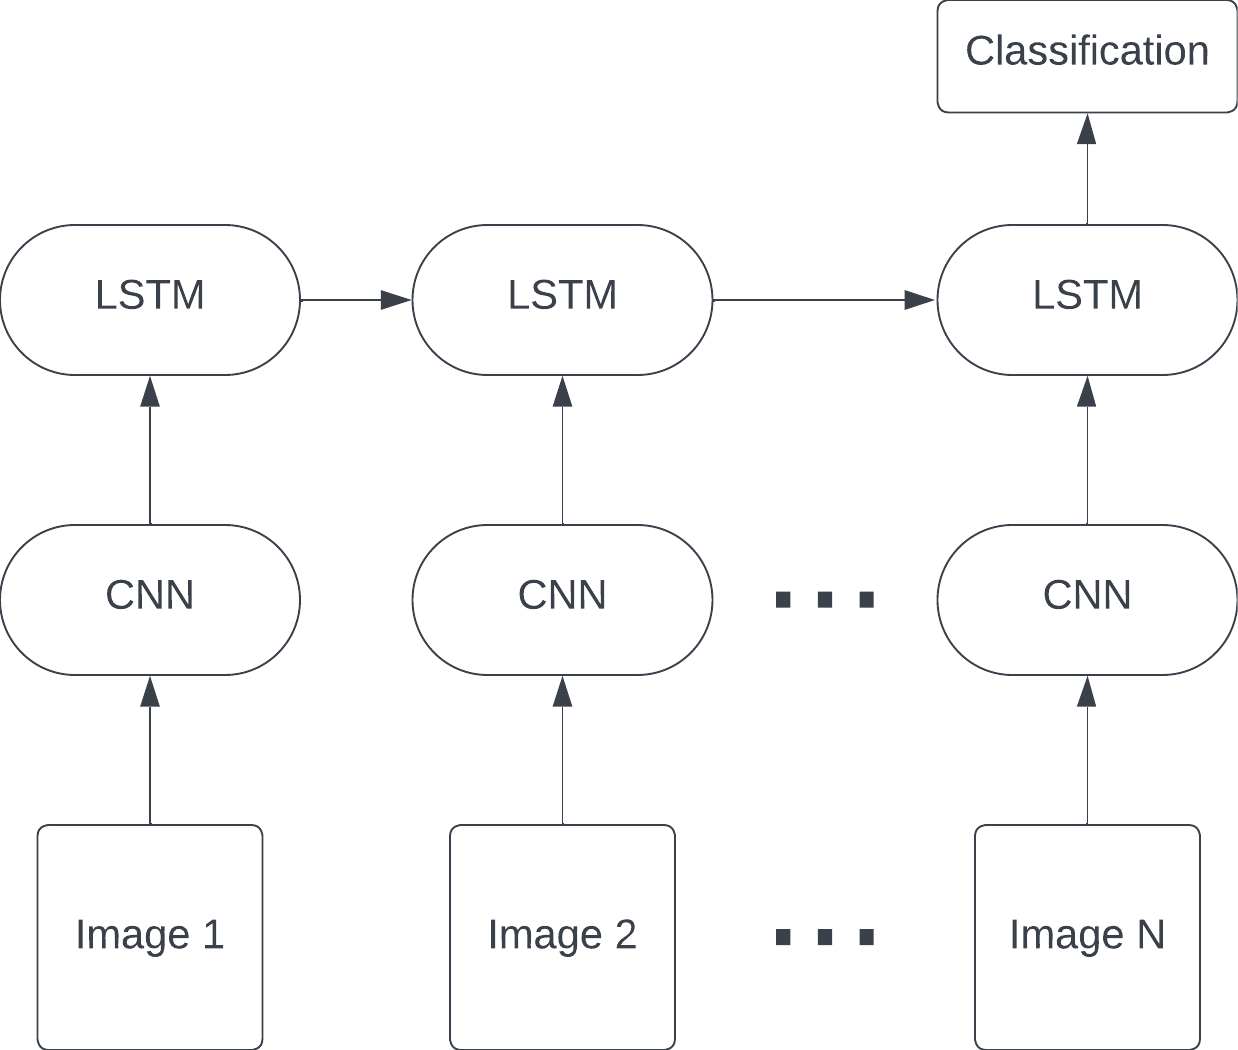
\includegraphics[width=8cm]{CNN-LSTM.png}
	\centering
	\caption{An example structure of a simple CNN-LSTM based model, each individual frame being individually fed into the CNN, and then passed to a LSTM.}
	\label{fig:cnn-lstm}
\end{figure}

The advantages of this model are that is is very lightweight and all of the individual parts are already well studied and efficient. This also means that the models are very lightweight, and relatively simple in comparison to more complex techniques.

The disadvantages of the model are also rooted in it's simplicity. The result of processing each image independently means that the interactions between frames is not very well represented. While the model is able to represent individual frame features very well, due to the fact that the feature maps are passed through the LSTM, classes that require specific movement from one frame to another are difficult to represent using this structure. Constructing these individual feature maps can also fall victim to background interference, meaning that a movement in the camera, or change in background could impact in a way that detracts from the main subject of the action more with this model than the other approaches discussed later in this chapter.

\begin{figure}[h]
	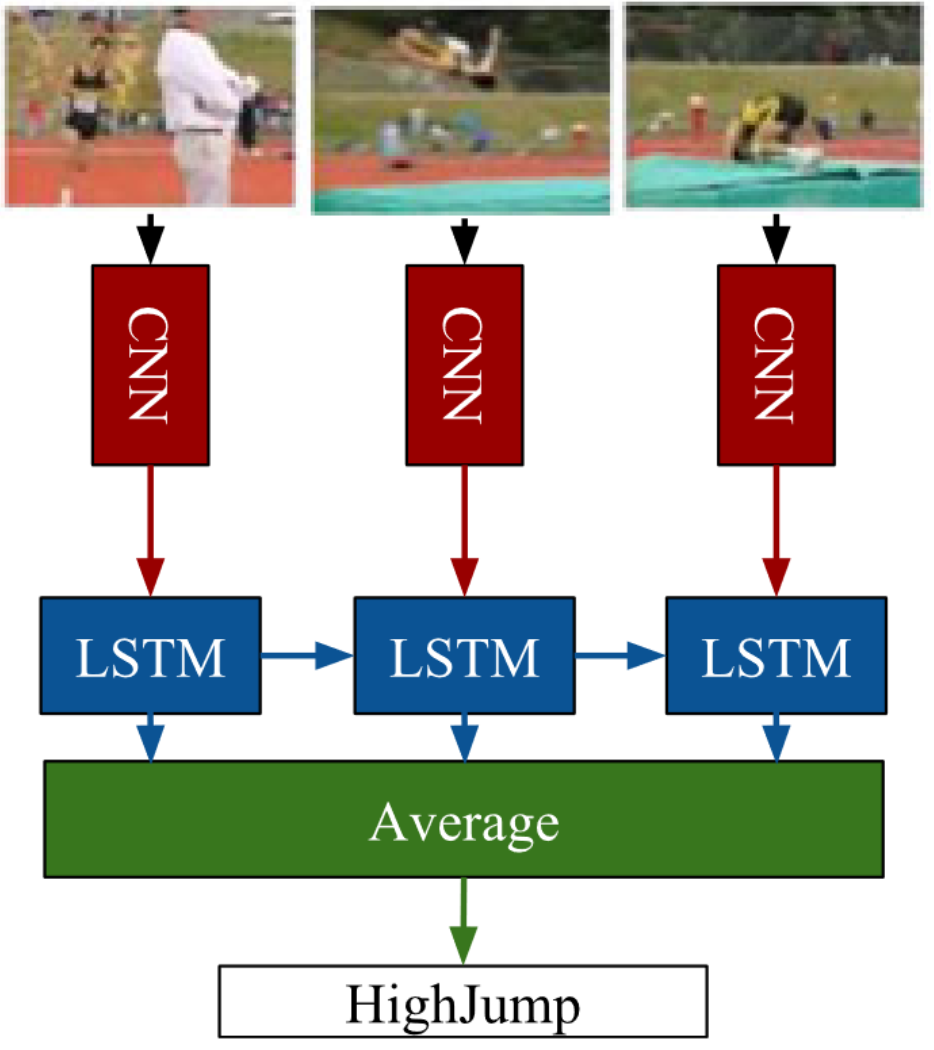
\includegraphics[width=8cm]{LRCN-AR.png}
	\centering
	\caption{Action recognition structure for the LRCN model. \cite{LRCNS}}
	\label{fig:lrcn-ar}
\end{figure}

\textbf{Long-term Recurrent Convolutional Networks} \cite{LRCNS}, is a model constructed using this methodology. In the paper, they use the notation that each frame, $x_{i}$, is fed into the CNN in order to construct a fixed-length feature representation, $\phi_{v}(x_{i})$. This is then passed into the recurrent sequence learning model. This is where the model differs from the previous example provided. In the LRCN model, the LSTM outputs at each frame are averaged to get the output class, rather than taking the last output. This removes any bias the model may have towards the later frames in long videos. In addition to RGB frames, this model additonally uses the optical flow feature, which easily adapts to this structure, replacing the RGB frames in figure \ref{fig:lrcn-ar}. The LSTM structure is taken from \cite{LSTM-2015}, which is a structure devised from the original LSTM model, as we discussed in section \ref{sec:LSTM}. The CNN's, represented in the paper as $\phi$, is described as a hybrid of the CaffeNet \cite{caffenet} (a variant of the AlexNet \cite{alexnet} model discussed in section \ref{sec:alexnet}) and the Zeiler and Fergus \cite{zeilerfergus} models, which has been pre-trained on a large dataset.

\begin{figure}[h]
	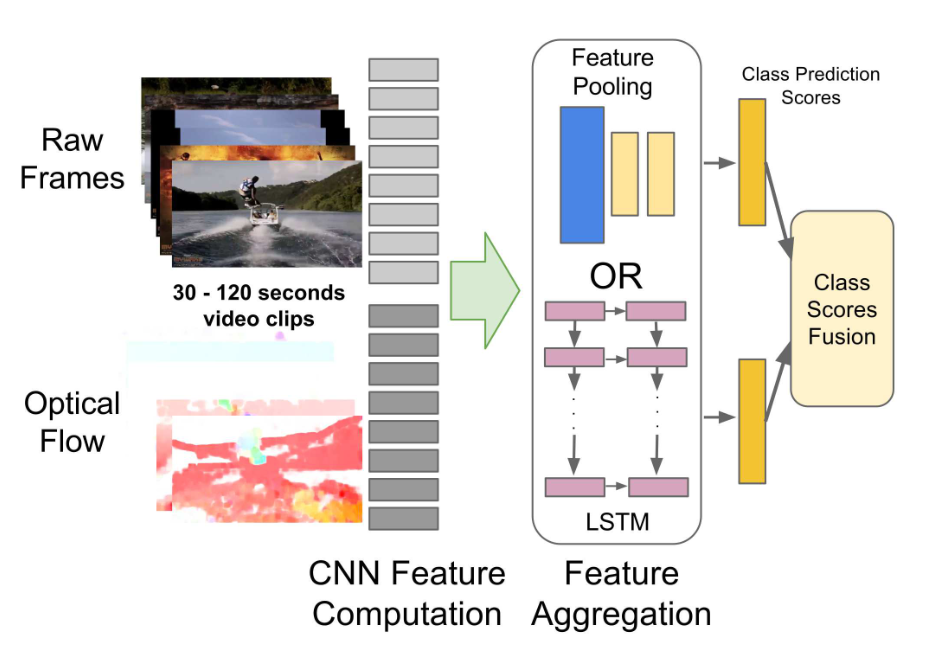
\includegraphics[width=10cm]{BeyondOverview.png}
	\centering
	\caption{Overview of the Beyond Short Snippets: Deep Networks for Video Classification model \cite{beyondshortsnippets}}
	\label{fig:beyondoverview}
\end{figure}

\textbf{Beyond Short Snippets: Deep Networks for Video Classification} \cite{beyondshortsnippets}, is another approach to this structure, which explores a more complex deep-LSTM based module, as well as more classical feature pooling. Similarly to the previously discussed model, Long-term Recurrent Convolutional Networks \cite{LRCNS}, the model utilizes a combination of two popular CNN models, AlexNet \cite{alexnet} and GoogLeNet \cite{googlenet}. The paper did explore many more classical feature pooling architectures, and were proven to have good results, however these techniques were outperformed by the LSTM model. The paper utilized a deep LSTM architecture for the feature aggregation step, shown in figure \ref{fig:deeplstm}, which further adds to it's complexity, moving it above the CNN-LSTM architectures described previously. In this deep-LSTM module, the outputs of each frame are passed into a LSTM module as in the previous model, but the ouputs are then passed up through 4 more stacked layers of LSTM's, after reaching softmax layers which are averaged to get an output. These 4 additional layers of LSTM's mean it is more able to infer data moving from one frame to another. This model additionally explored the uses of optical flow and found that it adds a great deal to the accuracy of the model.

\begin{figure}[h]
	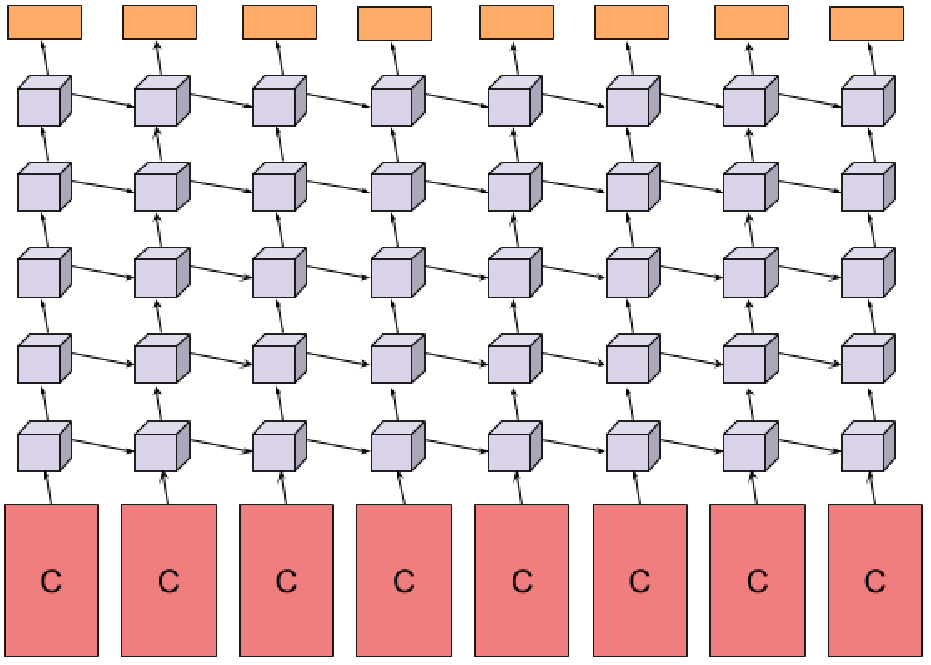
\includegraphics[width=8cm]{deepLSTM.png}
	\centering
	\caption{Deep LSTM architecture utilized by \cite{beyondshortsnippets} in the feature aggregation step as shown in figure \ref{fig:beyondoverview}.}
	\label{fig:deeplstm}
\end{figure}

%----------------------------------------------------------------------------------------
%	3D CNN
%----------------------------------------------------------------------------------------
\subsection{3D CNN Models}

When considering how to handle videos without the LSTM component, the most natural approach is to utilize 3 dimensional CNN kernels, the specifics of which were described in section \ref{3dkernels}. The function of these kernels when it relates to action recognition is that they allow for the model to easily encode local temporal data using the third kernel dimension. The primary issue with these models is that they contain many more parameters over the 2D CNN models, meaning that they take longer to train and require more computing power as compared to the lightweight counterparts.

\textbf{3D Convolutional Neural Networks for Human Action Recognition} \cite{3DCNN-ActionRecognition} was one of the original paper that proposed this model for the purposes of action recognition, and the greater topic of 3 dimensional convolutions as described in section \ref{3dkernels}. The general architecture of the model is shown in figure \ref{fig:original3dcnn}, and is very very similar to that of 2 dimensional CNNs, with convolutional layers followed up by subsampling layers.

\begin{figure}[h]
	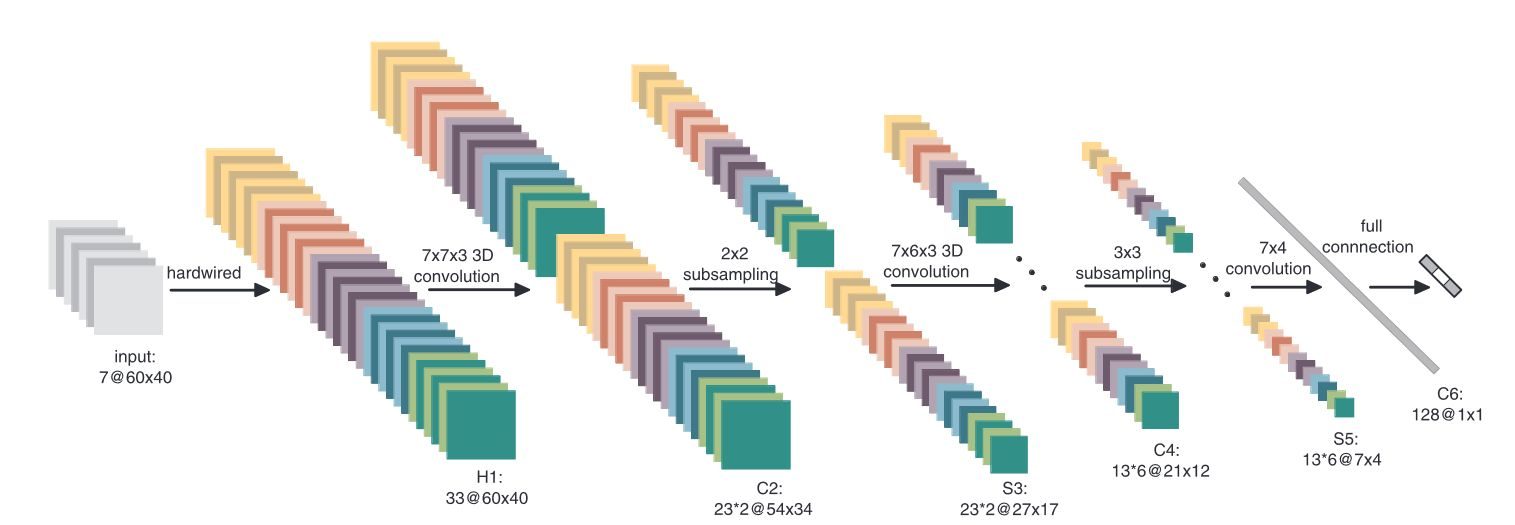
\includegraphics[width=10cm]{og3dCNN}
	\centering
	\caption{The original 3D-CNN action recognition model architecture proposed by \cite{3DCNN-ActionRecognition}, containing 3 convolutional layers, two subsampling layers, and one fully connected layer}
	\label{fig:original3dcnn}
\end{figure}

The primary difference with this original architecture compared to 2D CNN's as we know them today is that it used rather large $7x7x3$ convolutions, as compared to the typical $3x3$ convolutions used in classical 2D CNN's. \textbf{Learning Spatiotemporal Features with 3D Convolutional Networks} \cite{3x33dcnn}, is a slightly more modern architecture that was proposed. They explore in great detail the effects of these sizes of convolutions and find that this size of convolutions are more effective than the previous methods and sizes.

\textbf{Two-Stream Inflated 3D ConvNets}, commonly referred to as I3D \cite{i3d}, is a modern variation on 3D CNN based networks. Similar to the previously discussed model \cite{3DCNN-ActionRecognition}, this model explores the viability of taking techniques used in 2D CNN models and applying them to 3D. However it takes a much more direct approach, stating that they take the square filters of size $NxN$ and convert them simply to 3D filters with dimensions $NxNxN$, a process they describe as \textit{inflating} the convolutions. This inflation of convolutions allows for I3D to replicate successful 2D CNN's in their structure and apply them to video with little modifications.

\begin{figure}[h]
	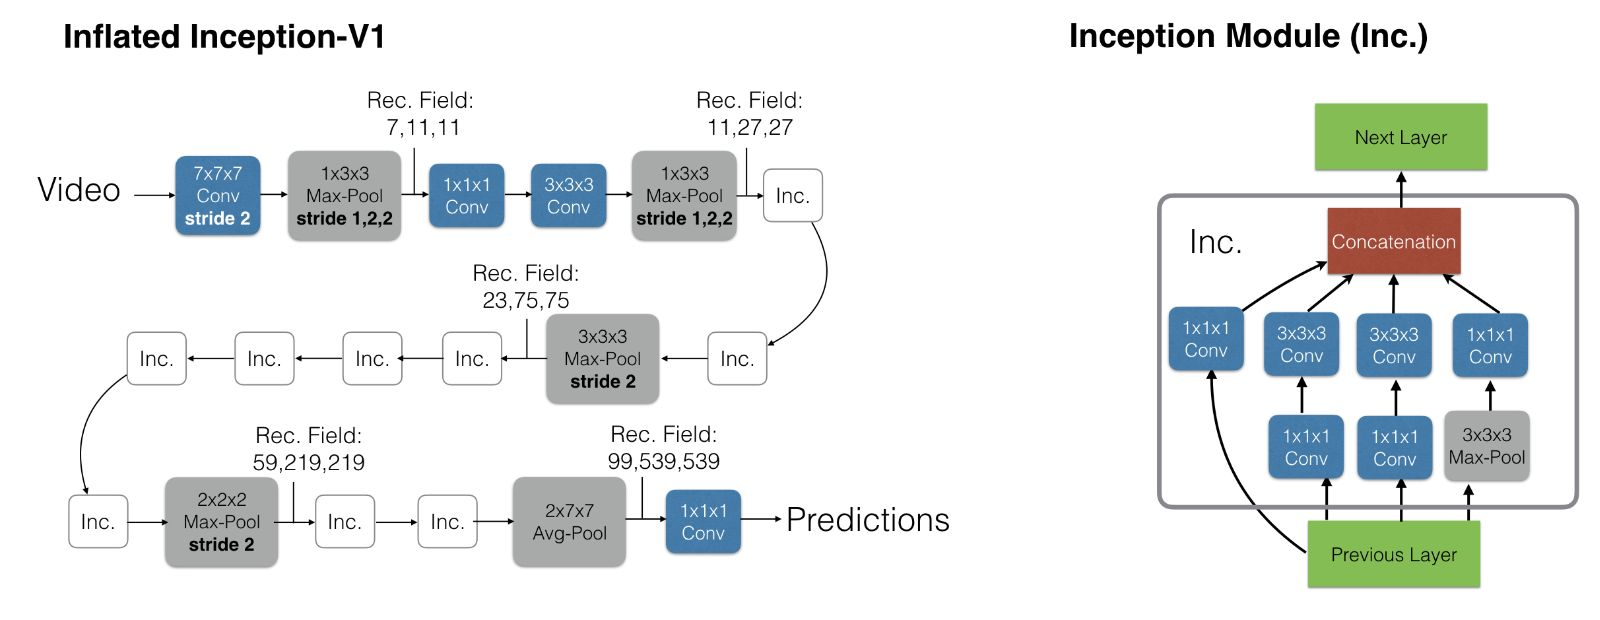
\includegraphics[width=15cm]{I3D}
	\centering
	\caption{The model architecture used in the I3D paper \cite{i3d}, where the Inflated Inception-V1 architecture (left) and it's detailed submodule (right) are shown.}
	\label{fig:I3D}
\end{figure}

%----------------------------------------------------------------------------------------
%	Modern
%----------------------------------------------------------------------------------------
\section{Model Evolution}

The domain of action recognition is always evolving, and it would not be a complete review of the literature without acknowledging other approaches that extend beyond the reach of this thesis.

\begin{figure}[h]
	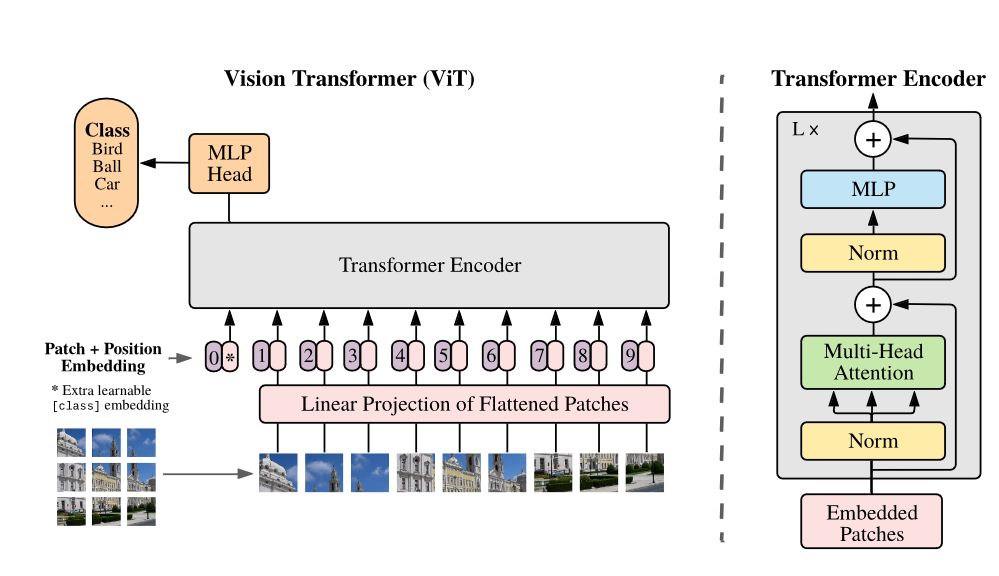
\includegraphics[width=10cm]{transformerActionRecognition}
	\centering
	\caption{The original transformer model proposed in \cite{transformer_og}, the image is split into fixed-size patches, linearly embed them, and add positional embeddings. It is then fed into a standard Transformer Encoder architecture.}
	\label{fig:transformerActionRecognition}
\end{figure}

\textbf{Transformers for Image Recognition at Scale} \cite{transformer_og}, extends beyond CNN's to explore transformer networks. While transformer networks are very easily applied to natural language processing tasks, it is not as easily applied to video and in particular action recognition. As depicted in figure \ref{fig:transformerActionRecognition}, the model utilizes a standard transformer architecture often used in NLP tasks in order to learn features that are useful for action recognition. The goal of this being to leverage previously well studied NLP studies that indicate the attention features of transformers are useful for focusing on the relevant data. Figure \ref{fig:attentionExample} shows this effect, the goal of this being to mitigate the challenges of handling background data interference as previously described in section \ref{sec:challenges}. This logic is then further expanded upon in many future models to extend this functionality, such as \textbf{Multiview Transformers for Video Recognition} \cite{multiview_transformers} which explores using multiple separate encoders to explore multiple views.

\begin{figure}[h]
	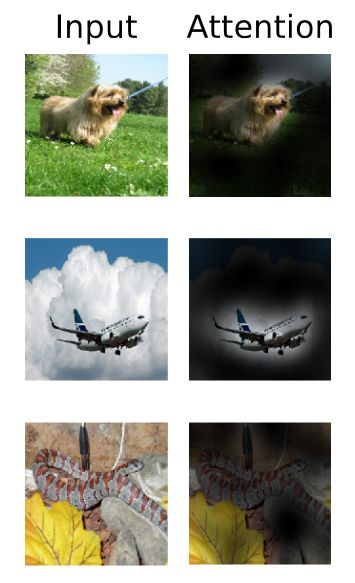
\includegraphics[width=5cm]{attentionExample}
	\centering
	\caption{Example feature outputs of how a transformer utilizes attention to focus on the main subject of a video in order to greater identify actions as shown in \cite{transformer_og}}
	\label{fig:attentionExample}
\end{figure}

%----------------------------------------------------------------------------------------
%	Datasets
%----------------------------------------------------------------------------------------
\section{Datasets}

\subsection{Kinetics}

\subsection{JHMDB}

%----------------------------------------------------------------------------------------
%	Pose Detection
%----------------------------------------------------------------------------------------
\section{Pose Detection}
\label{sec:pose-detection}

%----------------------------------------------------------------------------------------
%	Skeleton Based Models
%----------------------------------------------------------------------------------------
\section{Pose-Based Action Recognition}

Pose-based action recognition models have been well studied, and have been one of the popular forms of action recognition model. This is because by focusing on the pose (sometimes referred to as the skeleton) of the person, you are able to effectively mitigate the background effects that were discussed in section \ref{sec:challenges}. This means that typically more lightweight models can be used as they are able to be pointed more towards the main subject rather than filter out background data. Of course this method also comes with challenges, notably that in testing in the wild, there must be effectively two models, one to extract the pose from the person(s) in the frame, and one to process this pose data and export an action. This can introduce another point of failure, but as discussed in section \ref{sec:pose-detection}, 2D pose detection has been consistently improving to the point that high quality pose data from fast models is the norm.

\cite{WangPose} \cite{PCNN} \cite{Chained}

\cite{poseandjointaware}

\cite{smaller_faster_better}

\subsection{Intermediate Representations}

Intermediate representations are the vast majority of what will be discussed in later sections of this thesis. Intermediate representations aim to reduce the pose data that has been extracted into simpler and more processable formats. This is generally done with the aim of using a much more lightweight model (sometimes 2D CNN rather than 3D) that requires significantly less computing power. Of course this kind of pre-processing comes with issues, notably that by converting the model into a format such as this, some data will inevitably be lost during the transition, so the problem definition shifts slightly to creating an intermediate representation that both allows for a lightweight model to be effectively trained on it and for the smallest amount of data to be lost.

\cite{potion}

\cite{PA3D}

\cite{simple_yet_efficient}